\section{适定性}
\label{sec:pdeprob-well-posedness}

写出一个公式，是否就解决了问题？细棒的热方程反向求解也有“公式”：把初值的正弦系数乘上一个增长的指数，形式上和正向完全对称。下面会看到，这个公式几乎没有用处。判断一个问题是否提得合理，需要把三个问题分开回答。

\paragraph{三个问题}
把问题看成从数据到解的一个映射。这个映射要有意义，至少要回答：对给定的数据，解存在吗？解只有一个吗？数据有小的误差时，解的变化也小吗？这三个问题只有在明确了数据和解分别属于什么空间、用什么范数度量之后，才有确切的答案。

\begin{definition}[适定问题]
\label{def:pdeprob-well-posed}
设数据空间$D$和解空间$S$是赋范空间。若对每个$d\in D$，问题在$S$中存在唯一的解$\mathcal{S}(d)$，且映射$\mathcal{S}:D\to S$连续，即
\begin{equation}
  \lVert d_n-d\rVert_{D}\to0\ \Longrightarrow\ \lVert\mathcal{S}(d_n)-\mathcal{S}(d)\rVert_{S}\to0,
  \label{eq:pdeprob-continuous-dependence}
\end{equation}
就称问题在$(D,S)$下是\term{适定问题}（well-posed problem），否则称为\term{不适定问题}（ill-posed problem）。
\end{definition}

这是Hadamard提出的标准。线性问题中$\mathcal{S}$是线性映射，连续性等价于存在常数$C$，使得
\[
  \lVert\mathcal{S}(d)\rVert_{S}\leq C\lVert d\rVert_{D},\qquad\forall d\in D.
\]

图~\ref{fig:pdeprob-well-posed-map}画出了这三条要求：每个数据都有箭头指出（存在），箭头只有一支（唯一），数据的邻域映到解的小邻域（连续依赖）。线性算子方程的相应结论，可参考\BookChapterRef{chap:linear-operator-equations}{卷四第19章“线性算子方程”}。

\begin{BookInlineFigure}
  \centering
  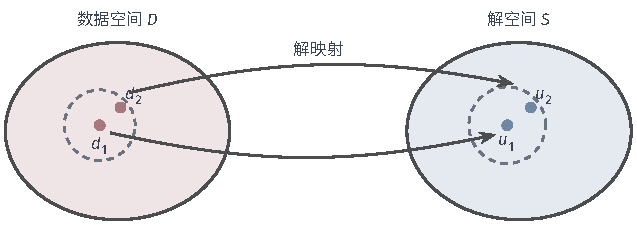
\includegraphics[width=107.8mm]{figures/06-differential-equations/02-partial-differential-equations/tikz/pdeprob-well-posed-map/figure.pdf}
  \caption{适定性是从数据空间到解空间的连续映射。虚线圈分别表示所选范数下的邻域，相近的数据$d_1,d_2$对应相近的解$u_1,u_2$。换一对空间，三条要求的答案都可能改变。}
  \label{fig:pdeprob-well-posed-map}
\end{BookInlineFigure}

\paragraph{存在：解空间是否够大}
存在性的答案依赖解空间。跳跃源项~\eqref{eq:pdeprob-step-source}在$C^{2}$中没有解，在$H_0^{1}$中有解；Neumann问题在数据违反式~\eqref{eq:pdeprob-neumann-compat}时哪里都没有解，这时要把数据空间缩小到满足约束的子空间。

非线性方程的存在性还有时间范围的问题。对Burgers方程，沿直线$x=x_0+u_0(x_0)t$，对$x_0$求导可得
\[
  \partial_xu=\frac{u_0'(x_0)}{1+u_0'(x_0)\,t}.
\]
只要某处$u_0'<0$，分母就会在有限时间变为零，光滑解只能存在到
\begin{equation}
  T^{*}=-\frac{1}{\min_xu_0'(x)}.
  \label{eq:pdeprob-burgers-breaking}
\end{equation}
式~\eqref{eq:pdeprob-burgers-ramp}的斜坡初值中$\min u_0'=-1$，$T^{*}=1$，与图~\ref{fig:pdeprob-burgers-crossing}一致。在$C^{1}$中只有局部解，放宽到弱解后解可以延续到所有时间。这和第~\ref{chap:ode-existence-continuation}章的情形类似，那里常微分方程的解也可能在有限时间爆炸，不过这里爆炸的是导数，而解本身仍然有界。

\paragraph{唯一：解空间是否够小}
解空间放得太大，唯一性就会失去，上一节的两个弱解和无穷多条锯齿线都是例子。Neumann问题差一个常数，这时要在解空间上加均值为零的条件，或者把差常数的函数视为同一个。

对线性演化方程，证明唯一性最常用的工具是能量估计：对两个解的差构造一个非负量，证明它不增。下面的定理同时给出唯一性和连续依赖。

\begin{theorem}[细棒热方程的能量估计]
\label{thm:pdeprob-heat-energy}
设$u_1,u_2$在$[0,1]\times[0,T]$上连续，$\partial_tu_i$、$\partial_xu_i$、$\partial_x^{2}u_i$在同一闭集上连续，满足同一方程$\partial_tu=\partial_x^{2}u+f$和同一边值$u(0,t)=g_0(t)$、$u(1,t)=g_1(t)$。则对$t\in[0,T]$，
\begin{equation}
  \lVert u_1(\cdot,t)-u_2(\cdot,t)\rVert_{L^{2}(0,1)}\leq\lVert u_1(\cdot,0)-u_2(\cdot,0)\rVert_{L^{2}(0,1)}.
  \label{eq:pdeprob-heat-energy}
\end{equation}
特别地，初值相同的两个解相等。
\end{theorem}

\begin{proof}
记$w=u_1-u_2$。由线性，$w$满足$\partial_tw=\partial_x^{2}w$，两端值为零。定义
\[
  E(t)=\frac12\int_0^{1}w(x,t)^{2}\,\mathrm{d}x.
\]
$\partial_tw$在闭集上连续，可以在积分号下求导，再代入方程：
\[
  E'(t)=\int_0^{1}w\,\partial_tw\,\mathrm{d}x=\int_0^{1}w\,\partial_x^{2}w\,\mathrm{d}x.
\]
分部积分，端点项$[w\,\partial_xw]_0^{1}$因$w$在两端为零而消失：
\[
  E'(t)=-\int_0^{1}(\partial_xw)^{2}\,\mathrm{d}x\leq0.
\]
所以$E(t)\leq E(0)$，开方即得式~\eqref{eq:pdeprob-heat-energy}。初值相同时$E(0)=0$，于是$E\equiv0$，$w\equiv0$。
\end{proof}

定理中的条件要求解光滑到初始时刻和边界。在无界区域上，单凭方程和初值并不能保证唯一性：实轴上的热方程存在初值为零、但不恒为零的解，它们在$\lvert x\rvert\to\infty$时增长得极快。这个构造由Tikhonov给出，证明需要较长的级数估计，读者可查阅偏微分方程教材。加上增长限制$\lvert u(x,t)\rvert\leq C\mathrm{e}^{ax^{2}}$后唯一性恢复，这说明解空间的限制不是技术细节。

\paragraph{连续依赖：同一方程，两个方向}
现在回到本节开头的问题。设$u_0=\sum_kb_k\sin k\pi x$，$u$是细棒两端为零的热方程的解，则第$k$个模式的系数在时刻$t$变为$b_k\mathrm{e}^{-k^{2}\pi^{2}t}$。由正弦函数的正交性，$\lVert\sin k\pi x\rVert_{L^{2}(0,1)}^{2}=\frac12$，于是
\[
  \lVert u(\cdot,T)\rVert_{L^{2}(0,1)}^{2}
  =\frac12\sum_kb_k^{2}\mathrm{e}^{-2k^{2}\pi^{2}T}
  \leq\lVert u_0\rVert_{L^{2}(0,1)}^{2}.
\]
正向映射$u_0\mapsto u(\cdot,T)$在$L^{2}$上有界，高频模式被强烈衰减。

反过来，由$T$时刻的温度$d=\sum_kd_k\sin k\pi x$推算初始温度，公式也可以写出来：
\begin{equation}
  u(x,0)=\sum_{k\geq1}d_k\,\mathrm{e}^{k^{2}\pi^{2}T}\sin k\pi x.
  \label{eq:pdeprob-backward-heat}
\end{equation}
形式上它和正向一样简单，但指数的符号反了。图~\ref{fig:pdeprob-backward-heat}(a)比较了两个方向上各模式的放大倍数。

这个公式首先不保证解存在。要让式~\eqref{eq:pdeprob-backward-heat}属于$L^{2}$，$d_k$必须满足$\sum_kd_k^{2}\mathrm{e}^{2k^{2}\pi^{2}T}<\infty$。折线$\min\{x,1-x\}$的系数只有$k^{-2}$的量级，不满足这个条件，它不可能是任何$L^{2}$初值在正时刻的温度。这和正向热方程瞬间变光滑是同一件事。

唯一性倒还成立：若$d=0$，每个$d_k$为零，$L^{2}$初值的所有系数都为零。问题出在连续依赖。取数据的扰动$\delta=\varepsilon\sin k\pi x$，它的$L^{2}$范数是$\varepsilon/\sqrt{2}$，反算出的初值扰动是
\[
  \varepsilon\,\mathrm{e}^{k^{2}\pi^{2}T}\sin k\pi x,
\]
放大倍数是$\mathrm{e}^{k^{2}\pi^{2}T}$，随$k$无界增长。所以反向映射在$L^{2}$上无界，问题在$(L^{2},L^{2})$下不适定。

下面取具体的数字。$T=0.1$，真实初值$\sin\pi x$，它在$T$时刻的温度是$\mathrm{e}^{-\pi^{2}T}\sin\pi x$。给这个数据加上幅度$\varepsilon=10^{-10}$的第$5$模式扰动，反算时模式$5$的放大倍数是
\[
  \mathrm{e}^{25\pi^{2}\cdot0.1}\approx5.2\times10^{10},
\]
反算结果中出现幅度约$5.2$的振荡。图~\ref{fig:pdeprob-backward-heat}(b)中，真实解的幅度为$1$，几乎完全被这个振荡淹没，而数据的扰动只有$10^{-10}$，小于任何测量误差。

\begin{BookInlineFigure}
  \centering
  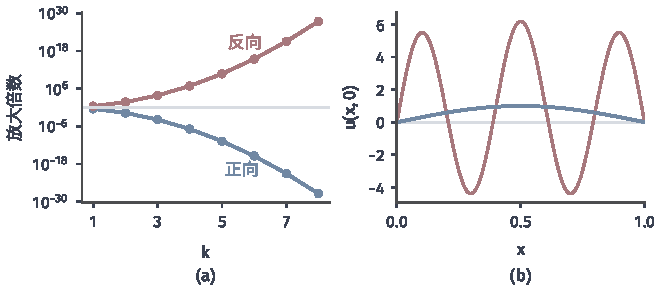
\includegraphics[width=112.0mm]{figures/06-differential-equations/02-partial-differential-equations/matplotlib/pdeprob-backward-heat/figure.pdf}
  \caption{热方程的两个方向，$T=0.1$。(a)第$k$个模式的放大倍数：正向$\mathrm{e}^{-k^2\pi^2T}$（蓝）与反向$\mathrm{e}^{k^2\pi^2T}$（红），纵轴为对数坐标。(b)真实初值$\sin\pi x$（蓝）与数据含幅度$10^{-10}$的第$5$模式扰动时的反算结果（红）。}
  \label{fig:pdeprob-backward-heat}
\end{BookInlineFigure}

适定性是相对于空间而言的，这里可以看得很清楚。若把数据空间的范数改为
\[
  \lVert d\rVert_{*}^{2}=\frac12\sum_kd_k^{2}\mathrm{e}^{2k^{2}\pi^{2}T},
\]
反向映射就成了等距映射，问题“适定”了。但这个范数下的小，意味着高频分量小到指数级，现实的测量误差达不到，这种适定性没有实用价值。选择空间时要问：数据的误差实际上在什么范数下小？

\paragraph{同一方程，换一种数据}
椭圆方程有一个著名的类似例子，说明同一方程配不同的数据，结果可以完全不同。考虑上半平面上的Laplace方程，把$y$当作“时间”，像波动方程那样给两个初值：
\begin{equation}
  \partial_x^{2}u+\partial_y^{2}u=0,\qquad
  u(x,0)=0,\qquad \partial_yu(x,0)=\frac{\sin kx}{k}.
  \label{eq:pdeprob-hadamard}
\end{equation}
直接代入可以验证，解是
\[
  u(x,y)=\frac{\sinh(ky)\sin kx}{k^{2}}.
\]

$k\to\infty$时，数据一致地趋于零，解却对每个$y>0$都按$\mathrm{e}^{ky}/(2k^{2})$爆炸。$k=20$时，数据的幅度只有$0.05$，在$y=1$处解的幅度是$\sinh(20)/400\approx6.1\times10^{5}$。图~\ref{fig:pdeprob-hadamard}画出了这种增长。若把数据换成$\sin(kx)/k^{m}$，数据的任意有限阶导数都趋于零，指数增长依然如故。

\begin{BookInlineFigure}
  \centering
  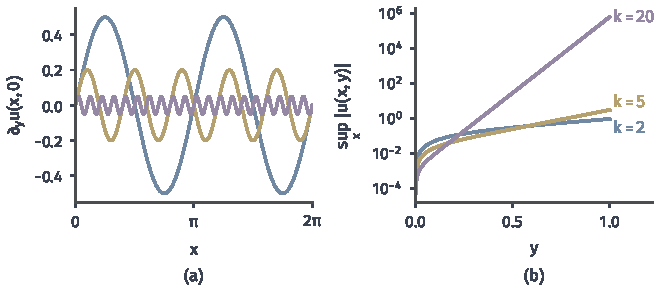
\includegraphics[width=112.0mm]{figures/06-differential-equations/02-partial-differential-equations/matplotlib/pdeprob-hadamard/figure.pdf}
  \caption{Laplace方程的“初值”问题~\eqref{eq:pdeprob-hadamard}。(a)数据$\partial_yu(x,0)=\sin(kx)/k$，$k=2$（蓝）、$5$（黄）、$20$（紫），频率越高幅度越小。(b)解的幅度$\sinh(ky)/k^2$随$y$的增长，纵轴为对数坐标。频率最高的数据最小，增长最快。}
  \label{fig:pdeprob-hadamard}
\end{BookInlineFigure}

同一方程配Dirichlet数据却是适定的。在$(0,1)$上取$-u''=f$，$u(0)=u(1)=0$，先对解本身做能量估计。将方程乘以$u$并分部积分，端点项消失：
\[
  \lVert u'\rVert_{L^{2}}^{2}=\int_0^{1}fu\,\mathrm{d}x\leq\lVert f\rVert_{L^{2}}\lVert u\rVert_{L^{2}}.
\]
再把$u$展开成正弦级数$\sum_kc_k\sin k\pi x$，由$k\geq1$，
\[
  \lVert u'\rVert_{L^{2}}^{2}=\frac12\sum_kk^{2}\pi^{2}c_k^{2}\geq\pi^{2}\lVert u\rVert_{L^{2}}^{2},
\]
这是区间上的Poincaré不等式。把它代入上式右端，两边约去$\lVert u'\rVert_{L^{2}}$，得到
\begin{equation}
  \lVert u'\rVert_{L^{2}(0,1)}\leq\frac{1}{\pi}\lVert f\rVert_{L^{2}(0,1)}.
  \label{eq:pdeprob-poisson-energy}
\end{equation}
取$u=\sin\pi x$，$f=\pi^{2}\sin\pi x$时，两边都是$\pi/\sqrt{2}$，等号成立。由线性，这个估计同时给出唯一性和对$f$的连续依赖，存在性由第~\ref{chap:elliptic-equations}章的变分方法给出。

波动方程的估计量不同。设$u$在$[0,1]\times[0,T]$上二阶连续可微，满足$\partial_t^{2}u=c^{2}\partial_x^{2}u$和零边值，定义能量
\[
  E(t)=\frac12\int_0^{1}\bigl((\partial_tu)^{2}+c^{2}(\partial_xu)^{2}\bigr)\,\mathrm{d}x.
\]
求导并对第二项分部积分，端点上$\partial_tu=0$，于是
\begin{equation}
  E'(t)=\int_0^{1}\partial_tu\,\bigl(\partial_t^{2}u-c^{2}\partial_x^{2}u\bigr)\,\mathrm{d}x=0.
  \label{eq:pdeprob-wave-energy}
\end{equation}
能量守恒，对时间的两个方向都成立，这正是波动方程可逆的反映。它要求数据是一对函数，数据空间自然取$H_0^{1}(0,1)\times L^{2}(0,1)$，而不是$L^{2}$。

\paragraph{不同数据要求下的结果}
表~\ref{tab:pdeprob-well-posed-summary}把本章的例子放在一起。前两行方程相同、方向相反，第三、四行方程相同、数据位置不同，每一行都要连同空间一起读。其中Laplace方程Cauchy问题的唯一性来自调和函数的解析性，Burgers方程熵解的结论在第~\ref{chap:scalar-conservation-laws}章讨论，这里只记录结果。

\begin{BookInlineTable}
  \centering
  \begin{tabular}{llll}
    \toprule
    问题与空间 & 存在 & 唯一 & 连续依赖\\
    \midrule
    热方程正向，$L^{2}$ & 有 & 有 & 有\\
    热方程反向，$L^{2}$ & 一般无 & 有 & 无\\
    Poisson，Dirichlet，$H_0^{1}$ & 有 & 有 & 有\\
    Laplace，Cauchy数据 & 一般无 & 有 & 无\\
    Poisson，Neumann & 需式~\eqref{eq:pdeprob-neumann-compat} & 差常数 & 商掉常数后有\\
    Burgers，$C^{1}$ & 仅到$T^{*}$ & 有 & 局部有\\
    Burgers，弱解 & 有 & 无 & 无从谈起\\
    Burgers，熵解 & 有 & 有 & 有\\
    \bottomrule
  \end{tabular}
  \caption{同一方程在不同数据与空间要求下的适定性。}
  \label{tab:pdeprob-well-posed-summary}
\end{BookInlineTable}

适定也不等于计算容易。连续依赖只说误差放大倍数有限，这个倍数可能很大；离散后的方程是否继承连续问题的稳定性，是另一个问题，要在第~\ref{chap:pde-numerical-methods}章对具体格式讨论。
